\documentclass[pdftex,12pt,letter]{article}
\usepackage[margin=0.75in]{geometry}
\usepackage{verbatim}
\usepackage{graphicx}
\usepackage{cite}
\usepackage[pdftex,pdfpagelabels,bookmarks,hyperindex,hyperfigures]{hyperref}

\bibliographystyle{unsrt}

\newcommand{\fixme}[1]{\textbf{FIXME: #1}}    


\title{Basic Requirements for the protoDUNE Raw Data Mangement System and its Possible Configuration}
\date{\today}
\author{M. Potekhin$^a$ and B. Viren$^a$\\
\ \\
$^a$\textit{Brookhaven National Laboratory, Upton NY}
}

\begin{document}
\maketitle

\begin{abstract}
The protoDUNE detectors (dual-phase NA02 and single-phase NA04)
require a number of systems in order to marshal raw data from
their respective DAQ to prompt processing and mass storage.  This
document provides a high-level description of essnetial functionality and
configuration of these systems.
\end{abstract}
\pagebreak
\tableofcontents

\pagebreak

\section{Introduction}
\subsection{The role of the Raw Data Management System}
This document sets forth a few requirements for a protoDUNE Raw Data Management System
(which will be referred to as \textbf{RDMS} for brevity in this text).  The system will receive the raw data from
two sources: Data Acquisition Systems for the NP02 Dual-Phase (DP) and NP04 Single-Phase (SP) DUNE prototype detectors.
It will provide support for prompt (``express streams'' and other) processing.  It will marshal the data to mass storage, first
to to the offline disk and then to the archive tape system at CERN. It will also transfer a copy to FNAL and potentially
to a few other sites in the US and Europe for production and analysis.

\subsection{Overview of the Data Flow}
Fig.\ref{fig:flow} shows an overview of the systems that will be required.

\begin{figure}[h]
  \centering
  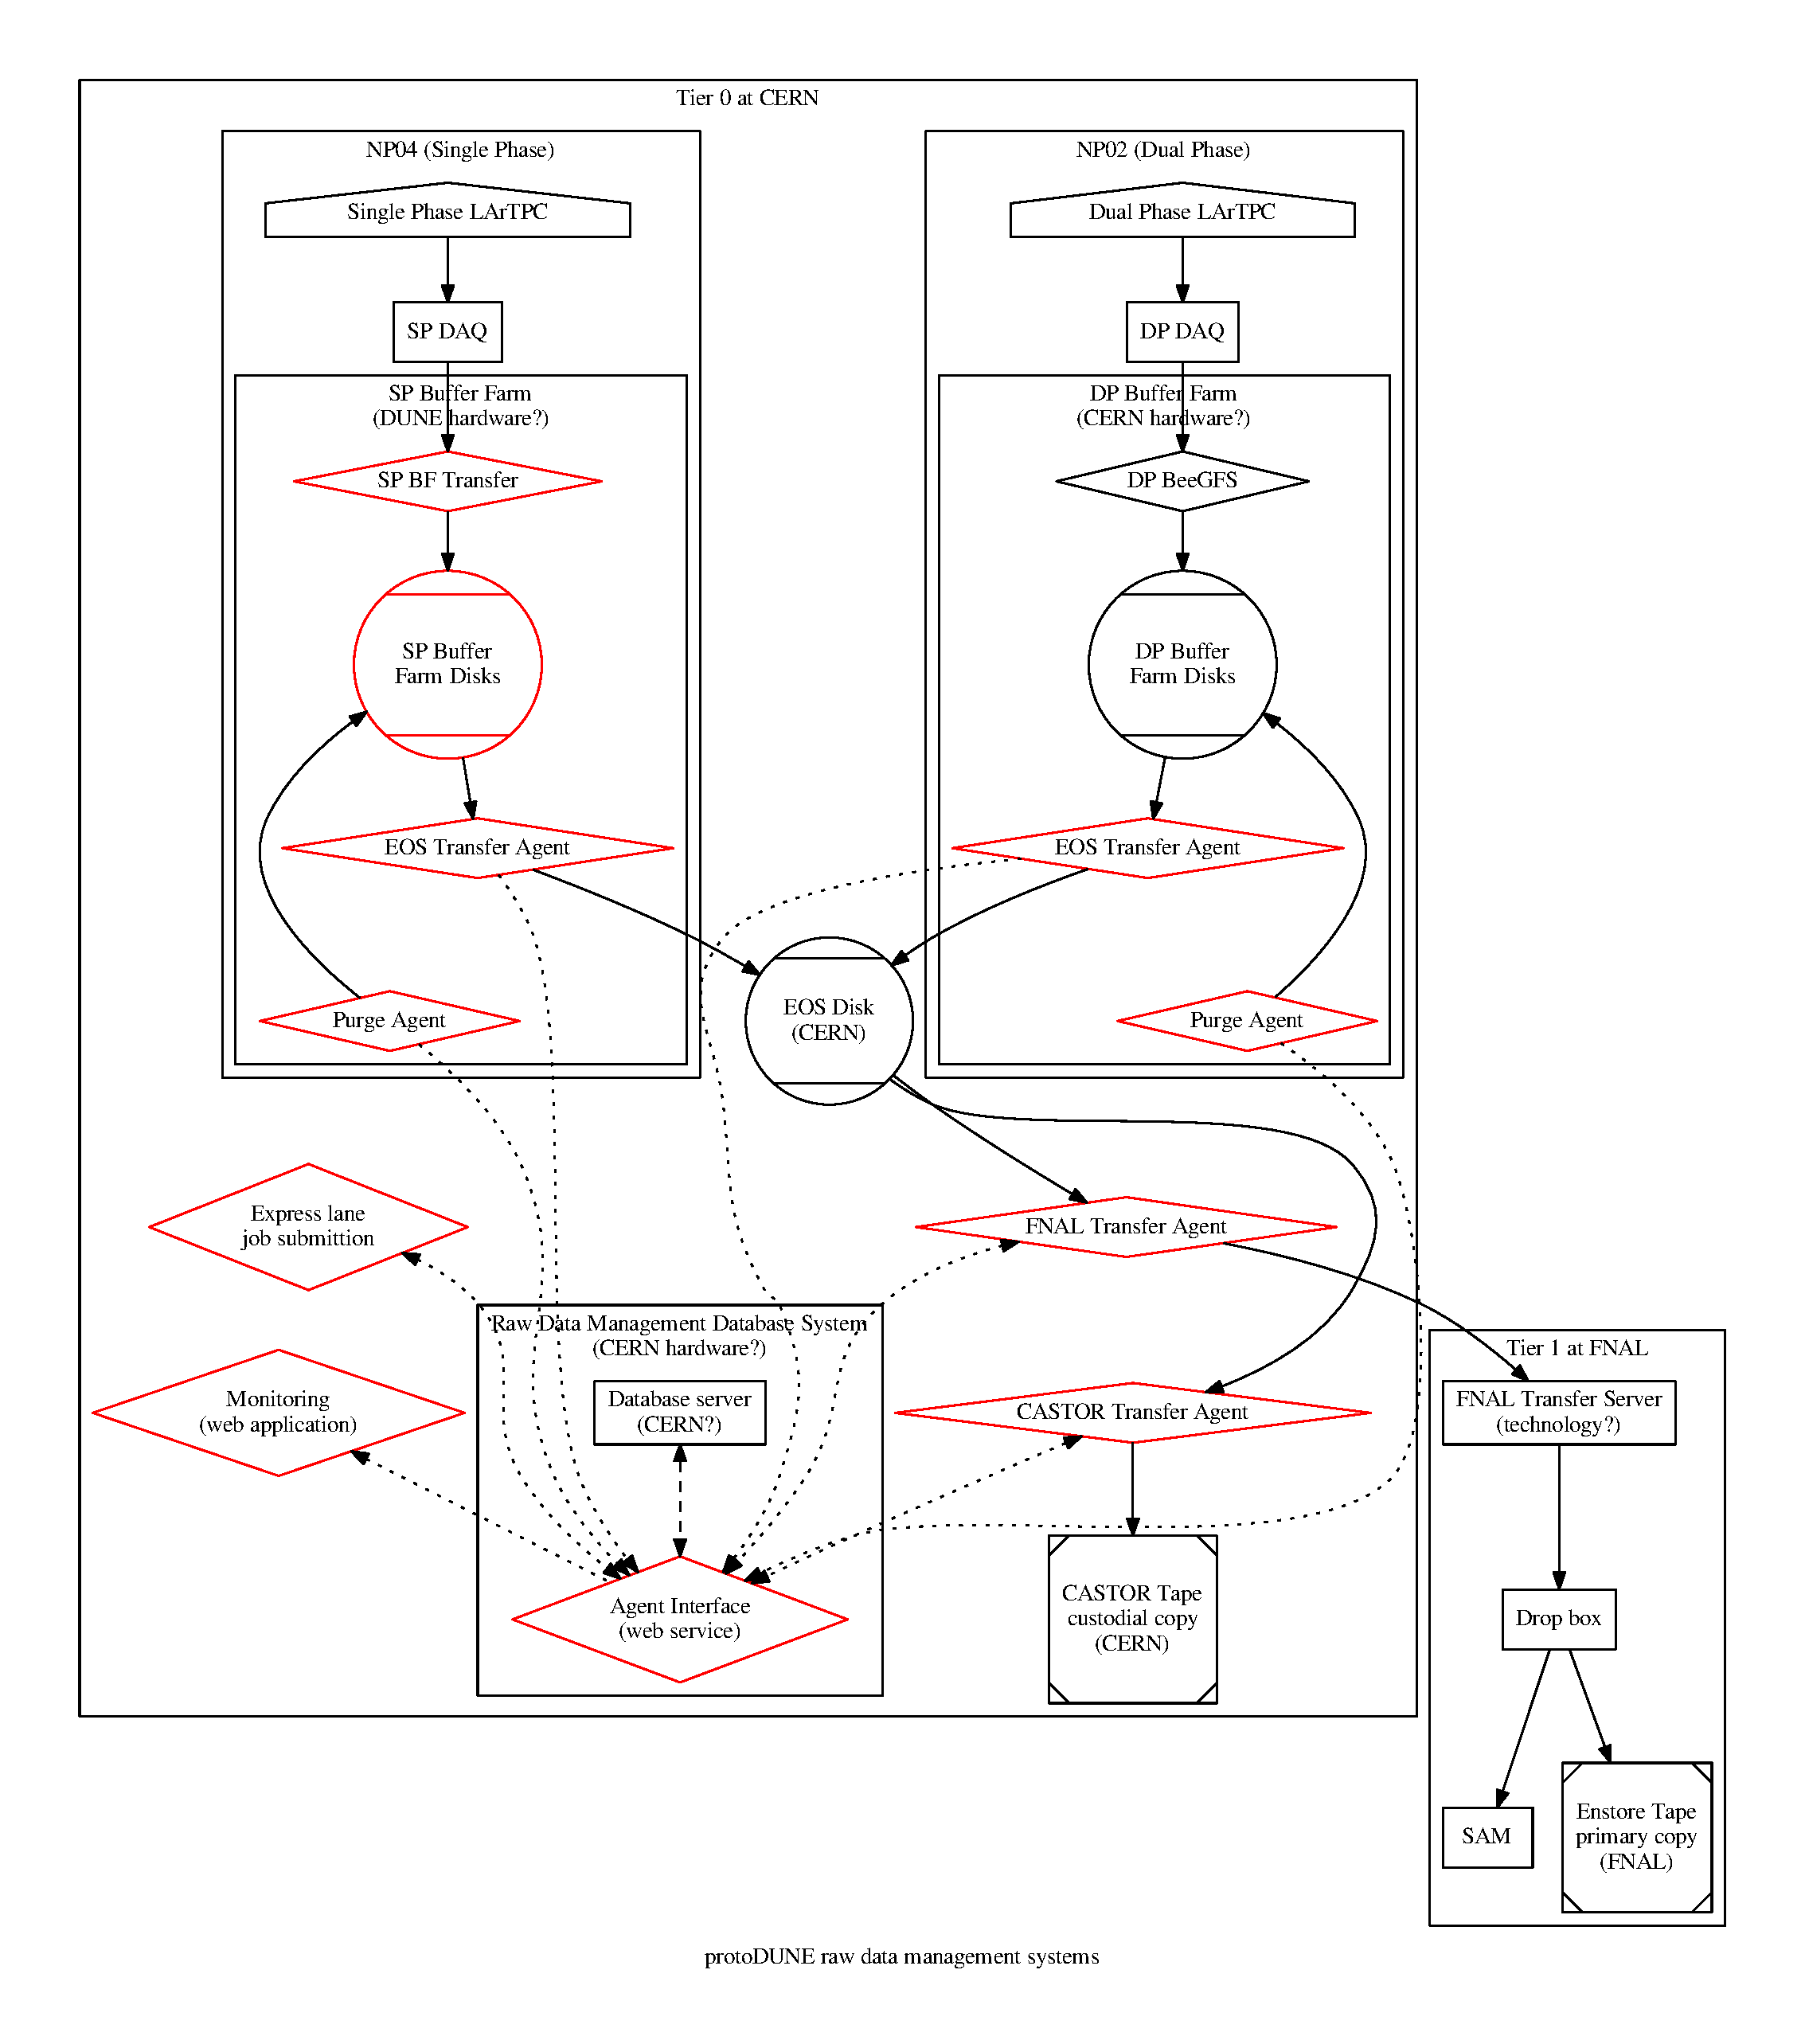
\includegraphics[width=0.75\textwidth]{flow.pdf}
  \caption{Systems required for protoDUNE raw data management.}
  \label{fig:flow}
\end{figure}

\noindent
In this diagram, red indicates systems where new development is needed.  Lined circles indicate disk and lined boxes indicate
tape storage hardware systems. Diamonds indicate software systems.  Solid arrows indicate flow of detector data, dotted
arrows indicate flow of metadata and dashed indicates database queries. In this scheme, the major hardware systems are:

\begin{description}
\item[Buffer Farms] each detector is expected to have a nearby and
  dedicated disk buffer farm
\item[RDM Server] hardware to run the RDM database and its Agent Interface.
\item[EOS \& CASTOR] CERN's disk and tape systems
\item[Enstore] FNAL's tape system

\end{description}

\noindent The major software systems are:

\begin{description}
\item[PDRDM] The protoDUNE Raw Data Management system is a central
  catalog for holding the state of all raw data files.
\item[agents] Various programs responsible for performing some action
  on a set of raw data files, potentially based on the state of the
  PDRDM and recording the outcome to the PDRDM system.
\end{description}

\noindent Details of these systems are given in the following sections.

\section{Hardware Systems}

\subsection{Buffer Farms}

It is assumed that each prototype detector has a nearby and dedicated
\textit{disk buffer farm} (BF).  They are required in order to isolate
online systems from offline ones.  Each BF is not necessarily expected
to be identical in terms of hardware characteristics or its software
because the two DAQs differ.  Their individual characteristics are:

\begin{description}
\item[DP buffer farm] configured with 1.4PB disk in 15 servers holding 16 disks each and 2x10GBE.~\cite{marteau}
\item[SP buffer farm] requires \fixme{XXX} TB distributed over
  \fixme{XXX} nodes with \fixme{XXX} bandwidth.  It is provided by
  \fixme{DUNE(?)}.
\end{description}

As described more in section~\ref{subsec:eosxferagent}, it is expected
that starting from the buffer farms the handling of the data from each
detector source will be symmetric in terms of what systems are
employed.  Other differences such as data rates, total volume, format
must be accommodated.

\subsection{EOS and CASTOR}

The EOS disk and CASTOR tape systems are expected to be provided by
CERN.  DUNE must estimate the required volume and bandwidth into each
of these systems (and out of EOS) for each detector individually and
should then negotiate with CERN to understand what is needed for them
to provide that.  DUNE should formulate an internal policy and
mechanisms to assure proper storage management and sharing so that
data from both prototypes can be accommodated.

\subsection{FNAL Ingest and Enstore}

The protoDUNE raw data management system will assure the raw data
files successfully reach Fermilab's transfer server.  Another system
is expected to then assure the data is properly cataloged and archived
to FNAL Enstore tape.  It is expected the same systems used for DUNE
35t and other Fermilab-based experiments will be used.  Specifically
the transfer server will deposit the accepted raw data files into a
``drop box''.  From there any metadata about the file will be inserted
into the SAM databas and the file itself archived to Enstore.

\section{Software Systems}

\subsection{DAQ-BF Transfer systems}

Raw data must be transferred from each detector DAQ to its respective
BF disk storage.  The general requirements of the DAQ-BF transfer
system are:

\begin{itemize}
\item must scale to provide required level of throughput from DAQ to disk.
\item integrating into developed DAQ software must not require
  substantial new effort.
\item the DAQ must not block while a transfer is ongoing such that it
  can not accept new data from readout electronics.
\end{itemize}

The transfer systems for the two detectors may differ.  Current
understanding and recommendations are summarized:

\begin{description}
\item[dual-phase] The DP detector has selected BeeGFS~\cite{beegfs}
  distributed, network file system for transferring data from DAQ to
  buffer disks.  

\item[single-phase] The SP detector requires development or adoption
  of a transfer method.  It is recommended to evaluate the technology
  adopted by DP and to evaluate XrootD~\cite{xrootd}
\end{description}

It is with files appearing on the respective BF that the protoDUNE Raw
Data Management (RDM) system takes over the provenance of the raw data
files.

\subsection{Raw Data Management System}

The protoDUNE RDM system is based on the idea of each file progressing
through a state machine of well defined states and explicit
transitions between those states.  State transitions are enacted by a
set of software agents.  The agent is required to perform an action
based on the current state of a file as set in the central RDM
database and record the outcome of the transition in said database.

Most agents will be written to perform a number of state transitions.
Some may inject initial state based on external information (eg, a
file appearing on a BF).  Other agents may merely monitor state
changes.  Figure~\ref{fig:flow} describes one possible set of agents.
As we learn more the set may grow with new functionality or splitting
large agents into smaller ones.  These agents are described in
section~\ref{subsec:agents}.

\subsection{Database}

The database is required to:
\begin{description}
\item[performance] accept new records at a rate on order of 10Hz and
  read-only queries an order of magnitude higher.
\item[schema] full history of inserts (no update nor delete of a
  previously inserted row), generate a unique identifier for each managed
  raw data file, relational associations to that ID.
\end{description}
The database is not directly exposed to agents but instead an Agent
Interface (RDM AI) is provided as an HTTP ``web service'' API,
described next


\subsection{Agent Interface}

The only direct access to the database should be through the Agent
Interface.  It is required to:
\begin{itemize}
\item present all database operations through a HTTP ``web service'' API.
\item expose functionality required by all expected agents as described below.
\item support and require authentication/authorization where needed.
\end{itemize}

All clients of the database shall use this interface, be they actually
effecting state changes or be they merely monitoring the state of the
database.

\subsection{Agents}
\label{subsec:agents}

Agents are expected to be command line programs or in some cases web
applications.  In general, they are required to:

\begin{itemize}
\item access and authenticate to the RDM AI
\item respect the allowed state transitions
\item report back on the outcome
\end{itemize}



\subsubsection{EOS Transfer Agent}
\label{subsec:eosxferagent}

The EOS Transfer Agent (ETA) is responsible for transferring files
from the BFs to EOS and recording the results.  Some detail will be
given here as a prototype for what must be given for all agents.

\begin{figure}[h]
  \centering
  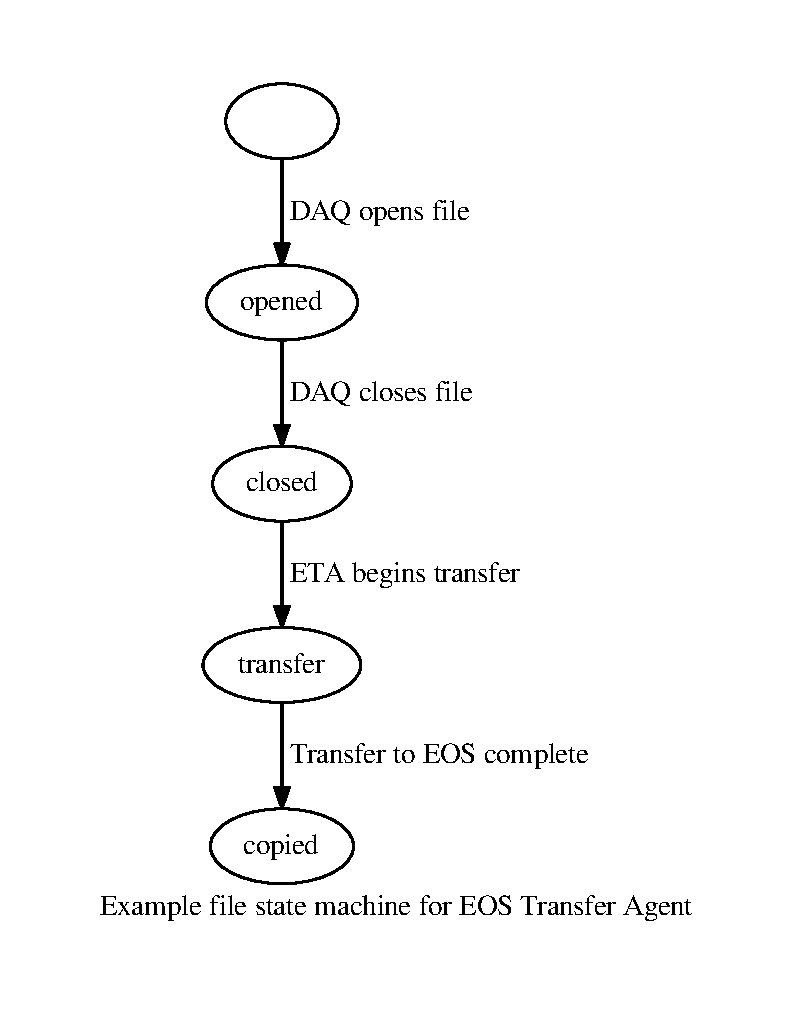
\includegraphics[width=0.5\textwidth]{state.pdf}
  \caption{EOS Transfer Agent states and transitions.}
  \label{fig:state}
\end{figure}

Figure~\ref{fig:state} gives the state machine implemented by the ETA.
This agent progresses sequentially through its possible states.  It
begins by watching its BF for the appearance of a new file and when
one appears it registers the file to the RDM DB via the AI that the
file is in state \texttt{opened}.  When it determines the DAQ has
finished writing the file this is registered as \texttt{closed} and a
transfer to EOS is begun with the equivalent \texttt{transfer} state
recorded.  When the transfer successfully concludes the
\texttt{copied} state is entered.

In addition to that behavior the ETA must
\begin{itemize}
\item be able to perform read and delete file operations on raw data
  files from both detectors BF disk storage
\item honor detector-specific policy regarding the timing of these
  file operations.
\item able to produce copies of raw files on EOS
\end{itemize}


\subsubsection{CASTOR Transfer Agent}

The CASTOR Transfer Agent (CTA) archives a file from EOS to CASTOR
tape.  It is required that the CTA:

\begin{itemize}
\item only archive a file that has reached the \texttt{copied} state
\item can read EOS file system and write to CASTOR
\end{itemize}

\subsubsection{Purge Agent}

The Purge Agent is responsible for deleting files when certain
conditions are met, depending on the context of the file to purge.
For example, BF files might only be purged after copied to EOS or they
may be delayed until archived to CASTOR.  A differently configured
Purge Agent may operate on files in EOS and purge based the file
reaching some appropriate state in the RDM DB.

\subsubsection{FNAL Transfer Agent}

The FNAL Transfer Agent (FTA) is responsible for transferring files
that have been copied to EOS to Fermilab via a to be determined
transfer server.  It is required to read EOS disk and connect to this
server.  

Once the transfer successfully complete, the fate of the raw file is
no longer the concern of the protoDUNE raw data management system.
Its continued management is taken over by systems at Fermilab.

\section{Summary and Future}

This report gives an outline for a design for a Raw Data Management
system for DUNE single-phase and dual-phase prototype detectors.  It
is based on agents enacting state changes on the files orchestrated by
a central database.  There are still many unknowns and gaps in the
design and it is expected that this document will be updated as the
design matures.  The design still needs to be presented to experts in
both SP and DP online, CERN and FNAL management and larger DUNE
collaboration.


\section{References}
\bibliography{citedb}


\end{document}

%%% Local Variables:
%%% mode: latex
%%% TeX-master: t
%%% End:
